% User Manual.tex

\documentclass[10pt]{article}
\usepackage[a4paper,left=1cm,right=1cm,top=1cm,bottom=1.5cm]{geometry}

\usepackage[T1]{fontenc} % an 8-bit encoding with 256 glyphs... because we can, and should!
\usepackage[scaled]{beramono} % bitstream vera mono, a good font for code
%\renewcommand*\familydefault{\ttdefault} % sets the document's font to the code's font
%\usepackage{indentfirst}
\setlength\parindent{0pt} % nothing will be indented
\usepackage{amsmath} % for math stuffs
\usepackage{graphicx, subfigure} % for images

% we use listings for the code examples
\usepackage{listings,color}
\usepackage[usenames]{xcolor}
% set up the listings
\lstset{
    language = Python,
    showstringspaces=false,
    formfeed=\newpage, % replaces formfeed character with newline when reading from .py files
    breaklines=true,
    tabsize=4,
    commentstyle=\itshape,
    basicstyle=\ttfamily, % use the beramono font
    moredelim=[il][\large\textbf]{\#\# },
    morekeywords={elif,sin,cos,tan,pi,integral,P1,P2,P3,HPR,text,format,time,slider,sliderP3,sliderHPR,sliderColor,Color,random,random01,randomRange,range,now,when,when1,react,react1,hold,key,to,at,itime,var,mouse,getX,getY,step,smoothStep,blastPicture,photoWheel,cube,tetrahedron},
    backgroundcolor=\color{lightgray}
}
%\lstset{numbers=right, numberstyle=\tiny, stepnumber=1, numbersep=5pt} % uncomment for line numbering

% creates a code command for loading examples from files (see use in Examples section)
\newcommand{\code}[2]{
    \hrulefill
    \subsection*{#1}
    \lstinputlisting{#2}
    \vspace{2em}
}

\renewcommand{\labelitemi}{} % this redefines the bullet macro used by itemize
\renewcommand{\labelitemii}{}
\renewcommand{\labelitemiii}{}
\renewcommand{\labelitemiv}{}

\title{Panda Camp User Manual}
\author{}
\date{}


\begin{document}
\maketitle



\section*{Introduction}
Camp philosophy; how should someone use this code.



\subsection*{Panda 3D}
Introduce Panda 3D and the reactive engine.



\section*{Math}
Explain the use of math in 3D environments and the engine.
\begin{itemize} % remove the '[]' to add bullets
    \item \underline{pi} - A value used to describe measures in radians.
    \item \underline{cos(a)} - A function that oscillates between -1 and 1 every 2pi units of time, starting at 0 (a = 0).
    \item \underline{sin(a)} - A function that oscillates between -1 and 1 every 2pi units of time, starting at 1 (a = 0).
    \item \underline{integral(a)} - This changes a speed (a) into a position.
\end{itemize}
The following sets the position of a panda using a speed while oscillating the HPR with sin and cos
\begin{lstlisting}
    p0 = P3(0, 0, 0)
    speed = P3(1, 0, 1)
    pos = p0 + integral(speed)
    panda(position = pos, hpr = HPR(sin(time), cos(time), 0))
\end{lstlisting}



\section*{Python}
What explanation should we give?
\begin{itemize}
    \item \underline{range(a, b)} - Returns a list of numbers between a lower bound (a) and upper bound (b).
    If only one parameter is given then 0 is the lower or upper bound.
%    \item \underline{random} - Python's random module has the following attributes
%    \begin{itemize}
%        \item \underline{.choose} - Chooses a random item from a list.
%    \end{itemize}
    \item \underline{randomRange(a, b)} - Generates a random number between a lower bound (a) and an upper bound (b).
    \item \underline{random01()} - Generates a random number between 0 and 1.
    \item \underline{for} - Allows you to do something more than once.
\end{itemize}
The following uses a for loop to generate 10 random numbers between 0 and 100
\begin{lstlisting}
    for i in range(10):
        print randomRange(0,100)
\end{lstlisting}
Loops can be nested for more complex tasks.
The following nests two loops to create a ten by ten grid of pandas
\begin{lstlisting}
    for i in range(10):
        for j in range(10):
            panda(position = P3(i, 0, j))
\end{lstlisting}
\begin{itemize}
    \item \underline{if} - A condition that, if met, causes something to happen.
    \item \underline{elif} - Another condition following an if or elif that, if met, causes something else to happen.
    \item \underline{else} - Causes something to happen only if the previous if and/or elif(s) aren't met.
\end{itemize}
\begin{lstlisting}
    if someBoolean: // this is the same as "someBoolean == True"
        // do something
    elif !someOtherBoolean: // this is the same as "someOtherBoolean != True"
        // do something else
    else:
        // if neither of the previous clauses hold
\end{lstlisting}
Discuss type casting and inference as well? What about recursion?

A function is how programmers are able to reuse code - do the same thing more than once, perhaps in slightly different ways.
Here is a function that creates a panda
\begin{lstlisting}
    def f(p):
        panda(position = p)
\end{lstlisting}
Here the argument p to the function f is a P3.
For further discussion of the use of functions see the Events and Reactions section.



\section*{Reactive}
Briefly describe what reactive code is in the context of the engine.
The following reactive variables are available
\begin{itemize}
    \item \underline{var(a)} - A reactive variable with an initial value a.
    This has the following reactive parameters
    \begin{itemize}
        \item \underline{.add(a)} - Adds a to the variable.
    \end{itemize}
    \item \underline{P3(x, y, z)} - Defines a location in 3-space.
    \item \underline{P2(x, y)} - Defines a location in 2-space (i.e. the surface of the screen)
    \item \underline{HPR(h, p, r)} - Determines the spin of an object using heading, pitch, and role; defines the objects orientation in 3-space
    \item \underline{Color(r, g, b)} - Defines color using the red (r), green (g), and blue (b) channels with values between 0 and 1 (see the ``Colors" section for a list of predefined colors)
    \item \underline{time} - A linear unit of measurement that begins when the program starts.
    This is variously used for movement and other reactive behavior.
    \item \underline{locelTime} - The time since an object has been created.
%    This can variously be used for movement as done here
%    \begin{lstlisting}
%        panda(position = P3(time, 0, 0), HPR(0, time, 0))
%    \end{lstlisting}
\end{itemize}



\section*{Non-Reactive}
Briefly describe what non-reactive code is in the context of the engine. Is there any worth mention? Is this section necessary?



\section*{Interface}
Describe the window that everything will run in and discuss the reactive stuffs that can be added.
\begin{itemize}
    \item \underline{text(a)} - Prints reactive and non-reactive types to the screen. This includes strings, floats, and P3s.
    \item \underline{format(s, a)} - This is used to combine strings (s) and other reactive and non-reactive variables (a) into a reactive form legible by text.
\end{itemize}
The following is an example of how to use text and format
\begin{lstlisting}
    text(format("You have scored %i in %f seconds", score, time))
\end{lstlisting}
Here \%i and \%f are conversion types, respectively representing the variables score (an int) and time (a float).
The following conversion types are available
\begin{itemize}
    \item \underline{i} - Signed integer.
    \item \underline{x} - Unsigned hexadecimal (lowercase).
    \item \underline{X} - Unsigned hexadecimal (uppercase).
    \item \underline{f} - Floating point (decimal format).
    \item \underline{c} - Single character (an integer or a single character string).
    \item \underline{r} - Converts any python object using repr().
    \item \underline{s} - Converts any python object using str().
\end{itemize}
Sliders are used to change the value a variable via the interface.
The following sliders are available
\begin{itemize}
    \item \underline{slider()} - Creates a slider that returns a floating point value.
    \item \underline{sliderP3()} - Creates a slider that returns P3 information.
    \item \underline{sliderHPR()} - Creates a slider that returns HPR information.
    \item \underline{sliderColor()} - Creates four sliders that set a color.
\end{itemize}
Sliders have the following parameters
\begin{itemize}
    \item \underline{label} (string, default value = None) - Text that will appear to the left of a slider.
    \item \underline{min} (float, default value = 0) - The minimum value of the slider (when it's all the way left).
    \item \underline{max} (float, default value = 1) - The maximum value of the slider (when it's all the way right).
    \item \underline{init} (float, default value = None) - The initial value of the slider.
    \item \underline{size} (float, default value = 1) - The size of the slider.
    \item \underline{position} (P3, default value = None) - Position on screen.
\end{itemize}
Here a slider is used to control the x-value of a panda's position
\begin{lstlisting}
    x = slider(label = "x-value", min = -3, max = 3, init = 0)
    panda(position = P3(x, 0, 0))
\end{lstlisting}
Here a color slider is used to change the background color of the world
\begin{lstlisting}
    color = sliderColor()
    world.color = color
\end{lstlisting}
\begin{itemize}
    \item \underline{check-boxes}?
    \item anything else?
\end{itemize}



\section*{Models}
%Describe what a model is: how it's made, brought into the engine, and how they're composed of reactive and non reactive components.
A model is a predefined object that appears on the screen whose representation is obtained from a 3D-model in an .eeg file.
By default the model is on the xy-plane facing in the y direction - towards the camera.
Models have the following reactive parameters
\begin{itemize}
    \item \underline{position} (P3, default value = P3(0, 0, 0)) - Location in 3-space.
    \item \underline{hpr} (HPR, default value = HPR(0, 0, 0)) - Orientation in 3-space.
    \item \underline{scale} (scalar, default value = 1 - 1 unit cube) - Relative scale.
    \item \underline{color} (Color, defule = None) - Blends a color with a models texture.
\end{itemize}
These parameters may be given values during initialization as follows
\begin{lstlisting}
    panda(position = P3(1, -2, 3.7), hpr = HPR(20, pi, time), scale = 0.76, color = Color(0, 0.3, random01())
\end{lstlisting}
They may also be given values after initialization by placing the model in a variable as follows
\begin{lstlisting}
    p = panda()
    p.position = P3(-3, 4, randomRange(-2, 4))
    p.hpr = HPR(cos(time), sin(time), 0)
    p.scale = sin(time)/3 + 1.2
    p.Color(0.45, 0.65, 0.23)
\end{lstlisting}
The value of these parameters may be retrieved at any time in a similar fashion.
The following places the following model's hpr on the screen
\begin{lstlisting}
    text(p.hpr)
\end{lstlisting}

Models have the following non-reactive variables
\begin{itemize}
    \item \underline{cRadius} (scalar) - The radius of the hypothetical cylinder that contains the model.
    \item \underline{cFloor} (scalar) - The position on the z-axis of the bottom of hypothetical cylinder that contains the model.
    \item \underline{cTop} (scalar) - The position on the z-axis of the top of hypothetical cylinder that contains the model.
    \item \underline{cType} (Type) - The model's type.
    \item \underline{duration} (scalar, defualt = None) - How long the model will remain on the screen.
    If None the model will not automatically disappear.
    \item \underline{collection} (Collection, default = None) - The collection the model belongs to.
\end{itemize}
A new variable can be added to a model on the fly as follows
\begin{lstlisting}
    p = panda()
    p.cute = True
\end{lstlisting}
Also, the following function is available for all models
\begin{itemize}
    \item \underline{pointForward(model)} - Points the model in the -y direction - the same as the camera by default - therefor forward.
\end{itemize}
%\subsection*{Predefined Models}
%\begin{figure}[h]
\begin{center}$
\begin{array}{ccc}
panda & ralph & sonic\\
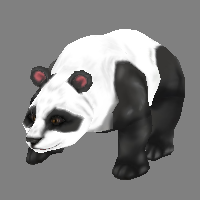
\includegraphics[width=1.5in]{images/models/panda.png} & 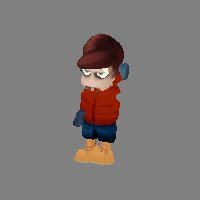
\includegraphics[width=1.5in]{images/models/ralph.png} & 
\includegraphics[width=1.5in]{images/models/sonic.png}\\
bender & sphere & soccerBall\\

\includegraphics[width=1.5in]{images/models/bender.png} & 
\includegraphics[width=1.5in]{images/models/sphere.png} & 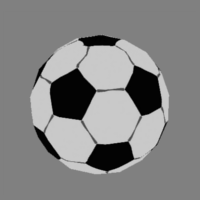
\includegraphics[width=1.5in]{images/models/soccerBall.png}\\
volleyBall & stretcher & gorilla\\
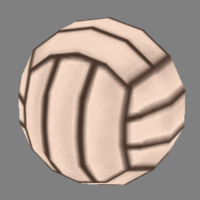
\includegraphics[width=1.5in]{images/models/volleyBall.png} & 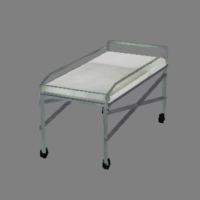
\includegraphics[width=1.5in]{images/models/stretcher.png} & 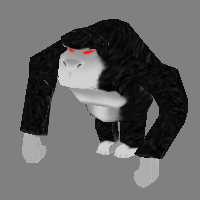
\includegraphics[width=1.5in]{images/models/gorilla.png}\\
bunny & r2d2 & girl\\
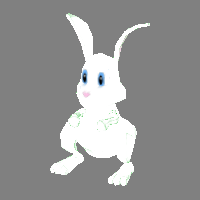
\includegraphics[width=1.5in]{images/models/bunny.png} & 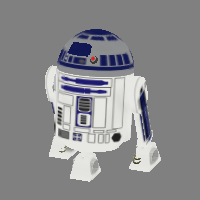
\includegraphics[width=1.5in]{images/models/r2d2.png} & 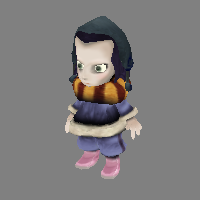
\includegraphics[width=1.5in]{images/models/girl.png}\\
\end{array}$
\end{center}
\begin{center}$
\begin{array}{ccc}
tails & truck & ford\\

\includegraphics[width=1.5in]{images/models/tails.png} & 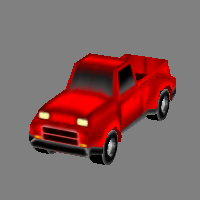
\includegraphics[width=1.5in]{images/models/truck.png} & 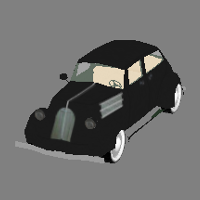
\includegraphics[width=1.5in]{images/models/ford.png}\\
jeep & boeing707 & blimp\\
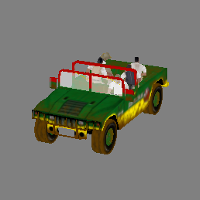
\includegraphics[width=1.5in]{images/models/jeep.png} & 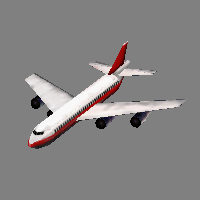
\includegraphics[width=1.5in]{images/models/boeing707.png} & 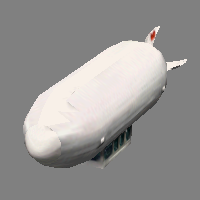
\includegraphics[width=1.5in]{images/models/blimp.png}\\
spaceship & hangGlider & russianBuilding\\
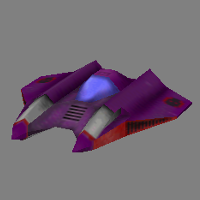
\includegraphics[width=1.5in]{images/models/spaceship.png} & 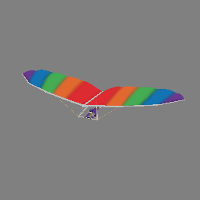
\includegraphics[width=1.5in]{images/models/hangGlider.png} & 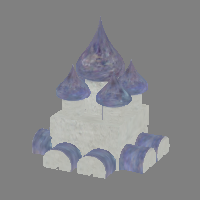
\includegraphics[width=1.5in]{images/models/russianBuilding.png}\\
\end{array}$
\end{center}
%\caption{Predefined Models}
%\end{figure}
%\begin{itemize}
%    \item panda
%    \item ralph
%    \item sonic
%    \item bender
%    \item sphere
%    \item soccerBall
%    \item volleyBall
%    \item stretcher
%    %\item chair % doesn't work
%    \item gorilla
%    \item bunny
%    %\item boyBalloon % doesn't work
%    \item r2d2
%    \item girl
%    \item tails
%    \item truck
%    \item ford
%    \item jeep
%    \item boeing707
%    \item blimp
%    \item spaceship
%    \item hangGlider
%    \item russianBuilding
%    \item discoHall
%    \item grassScene
%    \item trainEngineScene
%    \item forestSky
%    \item farmSky
%    \item sunset
%\end{itemize}



\section*{Rectangle}
Rectangles are geometric objects that are made using three points: lower-left, lower-right, and upper-left.
These are P3 points and are the only required parameters of the rectangle object.
Rectangles have the following optional properties
\begin{itemize}
    \item \underline{texture} (Color/texture, default value = None) - Used to set the color or the texture of the rectangle.
\end{itemize}
The color is set as follows
\begin{lstlisting}
    rectangle(P3(0, 0, 0), P3(1, 0, 0), P3(0, 1, 0), texture = purple)
\end{lstlisting}
A texture is an image and may be set like this
\begin{lstlisting}
    rectangle(P3(0, 0, 0), P3(1, 0, 0), P3(0, 1, 0), texture = "image.jpg")
\end{lstlisting}
\begin{itemize}
    \item \underline{side2} (Color/texture, defualt value = None) - Used to set the color or the texture of the back side of the rectangle.
    If left blank this will be the same color or texture as the front of the rectangle.
\end{itemize}
Like models, rectangles have the following parameters (see the Models section for the descriptions)
\begin{itemize}
    \item \underline{position}
    \item \underline{hpr}
    \item \underline{size} - This is synonymous to the models' \underline{scale} parameter.
    \item \underline{color}
\end{itemize}
Rectangles may be used to create various geometric solids as well.
\begin{itemize}
    \item \underline{blastPicture} - Takes a picture and slices it into smaller rectangles.
    Each of these rectangles has the following attributes
    \begin{itemize}
        \item \underline{.x} (float) - It's x position.
        \item \underline{.y} (float) - It's y position.
        \item \underline{.location} (P3) - It's location in 3-space.
    \end{itemize}
\end{itemize}
If a picture is blasted and each fragment's position is set to it's .location, the picture will be reassembled.
The following does just that and then spins the fragments 
\begin{lstlisting}
    fragments = blastPicture("image.jpg", 5, 5)

    for p in fragments:
        p.position = p.location
        p.hpr = HPR(time*random01(), 0, 0)
\end{lstlisting}
\begin{itemize}
    \item \underline{wheel} - Takes an arbitrary number of images as it's arguments and then uses them to create a wheel.
    \item \underline{cube} - Takes six images as it's arguments and places one on each side of a cube.
    \item \underline{tetrahedron} - Takes four images as it's arguments and places one on each side of a tetrahedron.
\end{itemize}
The following creates a wheel with five images
\begin{lstlisting}
    photoWheel(["image1.jpg", "image2.jpg", "image3.jpg", "image4.jpg", "image5.jpg"])
\end{lstlisting}



\section*{Movement}
Describe movement in a 3D environment (creating paths?)
\begin{itemize}
    \item \underline{step(a)} - A function that changes from 0 to 1 when the input (a) goes from positive to negative.
\end{itemize}
The following moves a panda after 2 seconds
\begin{lstlisting}
    panda(position = P3(step(time-2), 0, 0))
\end{lstlisting}
\begin{itemize}
    \item \underline{smoothStep} - The same as \underline{step} but smoothly steps rather than instantly stepping.
\end{itemize}
More complex paths can be created using the following interpolation functions
\begin{itemize}
    \item \underline{at(a)} - Puts the model at a given location (a - a P3).
    \item \underline{to(a, b)} - Moves the model to a location (b) over a given amount of time (a).
    \item \underline{itime(a)} - Uses the current time to select a place along the current path (a).
\end{itemize}
The following creates a path and moves a panda along it
\begin{lstlisting}
    p = panda()
    path = at(P3(0, 0, 0)) + to(1, P3(1, 0, 0)) + to(1, P3(-1, 0, 1))
    p.position = itime(path)
\end{lstlisting}



\section*{Controls}
The following reactive values are available to read user input
\begin{itemize}
    \item \underline{mouse} (P2) - Returns the position of the mouse with respect to the runtime window with values between -1 and 1, (0, 0) being the center.
    \item \underline{getX(mouse)} - Returns a floating point of the mouse's X value.
    \item \underline{getY(mouse)} - Returns a floating point of the mouse's Y value.
\end{itemize}
The mouse can be used to control the position of a panda as follows
\begin{lstlisting}
    panda(position = P3(getX(mouse), 0, getY(mouse)))
\end{lstlisting}
\begin{itemize}
    \item \underline{lbutton} (boolean) - Whether the left-mouse-button is pressed or not.
    \item \underline{rbutton} (boolean) - Whether the right-mouse-button is pressed or not.
\end{itemize}
An event is something that happens as the program runs, like mouse clicks and keys being pressed.
The following events are available
\begin{itemize}
    \item \underline{lbp} - Left-mouse-button pressed.
    \item \underline{rbp} - Right-mouse-button pressed.
    \item \underline{rbr} - Right-mouse-button released.
    \item \underline{lbr} - Left-mouse-button released.
\end{itemize}
These, and other keys, are given values using the following functions
\begin{itemize}
    \item \underline{key(a, b)} - Assigns the value b to the name a when a is pressed.
    \item \underline{keyUp(a, b)} - Assigns the value b to the name a when a is released.
\end{itemize}
The following are special key name
\begin{itemize}
    \item \underline{"f"+"1-12"} - These are the function keys, i.e. "f1", "f2", "f3", ... , "f12".
    \item \underline{"scroll\_lock"}
    \item \underline{"backspace"}
    \item \underline{"insert"}
    \item \underline{"home"}
    \item \underline{"page\_up"}
    \item \underline{"num\_lock"}
    \item \underline{"tab"}
    \item \underline{"delete"}
    \item \underline{"end"}
    \item \underline{"page\_down"}
    \item \underline{"caps\_lock"}
    \item \underline{"enter"}
    \item \underline{"arrow\_left"}
    \item \underline{"arrow\_up"}
    \item \underline{"arrow\_down"}
    \item \underline{"arrow\_right"}
    \item \underline{"shift"} - Either shift key.
    \item \underline{"lshift"} - Left-shift.
    \item \underline{"rshift"} - Right-shift.
    \item \underline{"control"} - Either control.
    \item \underline{"lcontrol"} - Left-control.
    \item \underline{"rcontrol"} - Right-control.
    \item \underline{"alt"} - Either alt.
    \item \underline{"lalt"} - Left-alt.
    \item \underline{"ralt"} - Right-alt.
    \item \underline{"space"}
\end{itemize}
An event can happen when more than one key is pressed.
An event can be composed of multiple keys using the + operator as follows
\begin{lstlisting}
    p = panda()
    v = hold(P3(0, 0, 0), key("left-arrow", P3(-1, 0, 0)) + key("right-arrow", P3(1, 0, 0)))
    p.position = P3(0, 0, -2) + integral(v)
\end{lstlisting}
    


\section*{Events and Reactions}
Discuss how events work (at a certain point in time) and why they're useful.
\begin{itemize}
    \item \underline{timeIs(a)} - Triggers when the time variable reaches a.
    \item \underline{now(a)} - Takes the value of a at that moment.
    \item \underline{hold(a, b)} - Holds the value a after the event b occurs.
    \item \underline{alarm(a)} - Generates an event at a given time step (a).
    \item \underline{happen(a, b)} - Turns a boolean a into an event b.
\end{itemize}
Discuss how reactions work and why they're useful.
Attach a reaction to a model by giving the triggering event and the name of the reaction function.
\begin{itemize}
    \item \underline{react(a, b)} - Calls the reaction b when the event a happens.
    \item \underline{react1(a, b)} - Same a react but it's reaction is the only executed code after the event.
\end{itemize}
Here is an example of using react with an alarm
\begin{lstlisting}
    a = alarm(step = 0.8)
    react(a, doSomething)
\end{lstlisting}
\begin{itemize}
    \item \underline{when(a, b)} - Same as react but happens when a condition a (true / false) is met.
    \item \underline{when1(a, b)} - The same as when but it's reaction is the only executed code after the event.
%    \item \underline{timer} - 
\end{itemize}



\section*{Particle Effects}
Particle effects are created much like models, having the same attributes and parameters.
The following particle effects are available.
\begin{itemize}
    \item \underline{intervalRings}
    \item \underline{likeFountainWater}
    \item \underline{shakenbSparkles}
    \item \underline{warpSpeed}
    \item \underline{heavySnow}
    \item \underline{lightSnow}
    \item \underline{explosions}
    \item \underline{fireWork}
    \item \underline{fireWorks}
    \item \underline{explosion}
    \item \underline{warpFace}
    \item \underline{fireish}
\end{itemize}



\section*{Camera}
%Talk about the camera.
The camera is how the scene is viewed.
By default the camera is on the xy-plane pointing in the -y direction - towards the models default position.
\begin{itemize}
    \item  \underline{mouseControlCamera(camera)} - Controls the camera using the mouse.
    \item \underline{.rod(a)} - This places the camera on a hypothetical rod behind an object (a), causing it to follow the object wherever it may go.
    It has the following parameters
    \begin{itemize}
        \item \underline{distance} (float, default value = 3) - Distance of the camera from the object.
        \item \underline{height} (float, default value = 0.5) - Height of camera off the xy-place.
    \end{itemize}
\end{itemize}



\section*{Light}
Describe the emulation of light in virtual worlds.
When no light source is specified, the world is filled with ambient light - light that comes from no particular direction.
By adding a light source, the ambient light is turned off.
The following light sources are available
\begin{itemize}
    \item \underline{pointLight} - Creates light from a single point.
    This has attributes similar to the models
    \begin{itemize}
        \item \underline{position} (P3)
        \item \underline{hpr} (HPR)
        \item \underline{color} (Color)
    \end{itemize}
    \item \underline{ambientLight} - This creates a light that comes from no particular direction.
    \item \underline{directionalLight} - Illuminates surfaces facing in the same direction identically.
    There are the following parameters
    \begin{itemize}
        \item um...
    \end{itemize}
\end{itemize}



\section*{Maps}
Describe maps and the various reactive and non-reactive components.



\section*{Sound}
Sound may be played in using the following methods
\begin{itemize}
    \item \underline{Sound(s)} - This creates a sound object that plays the sound file s.
    This object also has the following parameters
    \begin{itemize}
        \item \underline{loopCount} (int, default value = 1) - How many times the file will play.
        \item \underline{volume} (float, defauult value = 0.5) - The volume of the sound, 0 being mute and 1 being full.
    \end{itemize}
    \item \underline{play(s)} - Plays the sound file s once.
\end{itemize}



\section*{Useful Stuff}
This is where all the extra stuff goes.
\begin{itemize}
%    \item \underline{alarm}
    \item \underline{resetWorld()} - Removes everything from the world, interface objects included.
    \item \underline{collection} - A reactive group of objects?
%    \item \underline{var} - a reactive variable
%    \item \underline{localtime} - time that begins when an object is created
%    \item \underline{duration} - How long the object will be on the screen.
    \item \underline{exitScene()} - A reaction the removes a model from the world.
    \item \underline{HPRtpP3(a)} - Takes HPR a and converts it to a P3.
    \item \underline{P3toHPR(a)} - Takes P3 a and converts it to an HPR.
    \item \underline{P3C(a, b)} - Creates a P3 from cylindrical coordinates (angle a and length b)
\end{itemize}



\section*{Colors}
\begin{itemize}
    \item 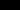
\includegraphics{images/colors/black.png} black
    \item 
\includegraphics{images/colors/blue.png} blue
    \item 
\includegraphics{images/colors/darkBlue.png} darkBlue
    \item 
\includegraphics{images/colors/lightBlue.png} lightBlue
    \item 
\includegraphics{images/colors/grey.png} grey
    \item 
\includegraphics{images/colors/gray.png} gray
    \item 
\includegraphics{images/colors/lightGray.png} lightGray
    \item 
\includegraphics{images/colors/darkGray.png} darkGray
    \item 
\includegraphics{images/colors/limeGreen.png} limeGreen
    \item 
\includegraphics{images/colors/green.png} green
    \item 
\includegraphics{images/colors/darkGreen.png} darkGreen
    \item 
\includegraphics{images/colors/hotpink.png} hotpink
    \item 
\includegraphics{images/colors/red.png} red
    \item 
\includegraphics{images/colors/darkRed.png} darkRed
    \item 
\includegraphics{images/colors/white.png} white
    \item 
\includegraphics{images/colors/yellow.png} yellow
    \item 
\includegraphics{images/colors/gold.png} gold
    \item 
\includegraphics{images/colors/silver.png} silver
    \item 
\includegraphics{images/colors/navyBlue.png} navyBlue
    \item 
\includegraphics{images/colors/purple.png} purple
    \item 
\includegraphics{images/colors/deepPurple.png} deepPurple
    \item 
\includegraphics{images/colors/violet.png} violet
    \item 
\includegraphics{images/colors/brown.png} brown
    \item 
\includegraphics{images/colors/orange.png} orange
    \item 
\includegraphics{images/colors/teal.png} teal
    \item 
\includegraphics{images/colors/cyan.png} cyan
    \item 
\includegraphics{images/colors/aquamarine.png} aquamarine
    \item 
\includegraphics{images/colors/slateGray.png} slateGray
    \item 
\includegraphics{images/colors/purpleBlue.png} deepPurple
    \item \includegraphics{images/colors/bloodOrange.png} bloodOrange
    \item \includegraphics{images/colors/fuchsia.png} fuchsia
    \item \includegraphics{images/colors/tan.png} tan
    \item \includegraphics{images/colors/lightTan.png} lightTan
    \item \includegraphics{images/colors/olive.png} olive
    \item \includegraphics{images/colors/springGreen.png} springGreen
    \item \includegraphics{images/colors/coral.png} coral
    \item \includegraphics{images/colors/salmon.png} salmon
    \item \includegraphics{images/colors/lavender.png} lavender
\end{itemize}



\section*{Examples}
Give some neat examples that draw on the content of the manual.

Here's a demonstration of a code example from a file.

\code{Code Example Name}{examples/demo.py}



\end{document}
